\documentclass{article}

% Symbols
\usepackage{amsfonts, amsthm}
\usepackage{upgreek}
\usepackage{physics}
\usepackage{cancel}
\usepackage{amssymb, latexsym, amsmath}
\usepackage{ stmaryrd }

%Algorithms
\usepackage[ruled,lined,linesnumbered,commentsnumbered]{algorithm2e}

%% Identación
\setlength{\parindent}{0cm}

% Comentario en bloques:
\iffalse
\fi

% Hipervínculos:
\usepackage{hyperref}

% Código
\newcommand{\code}[1]{\textcolor{white!25!black}{\texttt{#1}}}
\usepackage{listings}

%AMS
\usepackage{amsthm}
\newtheorem{algo-thm}{Algoritmo}

% Proof
\renewcommand*{\proofname}{\textbf{Demostraci\'on:}}
% Theorem
\newtheorem*{theorem}{Teorema}

% Graphics
\usepackage{graphicx}
\usepackage{pgf}

% Color a letras.
%\usepackage[usenames,dvipsnames,svgnames,table]{xcolor}

% Tikz
\usepackage{tkz-graph}
\usepackage{tikz}
\usetikzlibrary{arrows,automata}
\usepackage{tikz}
\usetikzlibrary{arrows,automata}
%\usetikzlibrary[topaths]
\usetikzlibrary{angles, quotes}
\usepackage{siunitx}

% Def. Dr. César.
\usetikzlibrary{shapes,calc}
\tikzstyle{edge}=[shorten <=2pt, shorten >=2pt, >=stealth, line width=1.1pt]
\tikzstyle{edgeDotted}=[shorten <=2pt, shorten >=2pt, >=stealth, line width=1.1pt, dashed] %  dashed
\tikzstyle{edgeC}=[curve to, out=270,in=270,relative, dashed]
\tikzstyle{blueE}=[shorten <=2pt, shorten >=2pt, >=stealth, line width=1.5pt, blue]
\tikzstyle{redE}=[shorten <=2pt, shorten >=2pt, >=stealth, line width=1.5pt, red]
\tikzstyle{blackV}=[circle, fill=black, minimum size=6pt, inner sep=0pt, outer sep=0pt]
\tikzstyle{brownV}=[circle, fill=brown, draw, minimum size=6pt, line width=0.75pt, inner sep=0pt, outer sep=0pt]
\tikzstyle{blueV}=[circle, fill=blue, draw, minimum size=6pt, line width=0.75pt, inner sep=0pt, outer sep=0pt]
\tikzstyle{redV}=[circle, fill=red, draw, minimum size=6pt, line width=0.75pt, inner sep=0pt, outer sep=0pt]
\tikzstyle{redSV}=[semicircle, fill=red, minimum size=3pt, inner sep=0pt, outer sep=0pt, rotate=225]
\tikzstyle{blueSV}=[semicircle, fill=blue, minimum size=3pt, inner sep=0pt, outer sep=0pt, rotate=225]
\tikzstyle{blackSV}=[semicircle, fill=black, minimum size=3pt, inner sep=0pt, outer sep=0pt, rotate=225]
\tikzstyle{vertex}=[circle, draw, minimum size=6pt, line width=0.75pt, inner sep=0pt, outer sep=0pt]

%%%%%%%%%%%%%%%%%%%%%%%%%%%%%%%%%%%%%%%%%%%%%%%%%%%%%%%%%
\newcommand\Star[3][]{%
\path[#1] (0  :#3) -- ( 36:#2) 
       -- (72 :#3) -- (108:#2)
       -- (144:#3) -- (180:#2)
       -- (216:#3) -- (252:#2)
       -- (288:#3) -- (324:#2)--cycle;}
%%%%%%%%%%%%%%%%%%%%%%%%%%%%%%%%%%%%%%%%%%%%%%%%%%%%%%%%%
% Margins
\addtolength{\voffset}{-1.5cm}
\addtolength{\hoffset}{-1.5cm}
\addtolength{\textwidth}{3cm}
\addtolength{\textheight}{3cm}

% Columnas multiples
\usepackage{multicol}

%Header-Footer
\usepackage{fancyhdr}
\renewcommand{\headrulewidth}{1pt}

\newcommand{\set}[1]{
  \left\{ #1 \right\}
}

%\pagenumbering{gobble} -- Este comando
%                       -- quita el número de página.
\footskip = 50pt
\renewcommand{\headrulewidth}{1pt}

\pagestyle{fancyplain}

\begin{document}
\title{UNIVERSIDAD NACIONAL AUT\'ONOMA DE M\'EXICO\\ Facultad de Ciencias}
\author{Autor: Adri\'an Aguilera Moreno}
\date{}
\maketitle
\begin{center}
  \includegraphics[scale=0.20]{../Imagen/Portada.jpg}\\[0.4cm]
  \Large
  \bf{Geometría Computacional}
  \normalsize
\end{center}
\newpage
\fancyhead[r]{ Geometría Computacional.}
%%%%%%%%%%%%%%%%%%%%%%%%%%%%%%%%%%%%%%%%%%%%%%%%%%%%%
\section*{\LARGE{Tarea 02}}
%%%%%%%%%%%%%%%%%%%% Problema01:
\textbf{1.} Sea $P$ un polígono convexo de $n$ vértices.
Suponga que los vértices de $P$ son dados en un arreglo
ordenado. Muestra que, dado unpunto $q$, podemos detectar
si $q \in P$ en tiempo $\mathcal{O}(\log n)$.

\begin{proof}
  Exhibamos un algoritmo en tiempo $\mathcal{O}(\log n)$
  para encontrar que $q \in P$. Esto lo podemos hacer
  de varias maneras, en partícular podemos usar una de
  las estructuras de datos vistas en clase o podemos
  usar una técnica basa en búsqueda binaria. Por simplicidad
  usaré la técnica basada en búsqueda binaria, a continuación
  se muestra el algoritmo deseado:
  \begin{enumerate}
  \item Encontremos el extremo ``más alto'' (digamos $a$) y
    ``más bajo'' (digamos $b$) en $P$ en $\mathcal{O}(1)$,
    pues tenemos los puntos ordenados en un arreglo.
  \item Verificamor que $b.y \leq q.y \leq a.y$ en $\mathcal{O}(1)$.
    Si la condición anterior se cumple, entonces seguimos con
    el algoritmo. Si no se cumple la condición anterior, entonces
    concluimos que $q$ no se encuentra destro de $P$.
  \item Ahora tracemos una recta $\ell$ a partir de $q$ tal que intersecte al
    polígono $P$ respecto a una proyección, digamos la proyección hacia la izquierda.
    Ahora, tendremos tres posibles opciones:
    \begin{enumerate}
    \item $\ell$ intersecta en $0$ puntos (Caso análogo a $2$). Entonces $q \notin P$.
    \item $\ell$ intersecta en $2$ puntos (Caso análogo a $1$). Entonces $q \notin P$.
    \item $\ell$ intersecta en $1$ punto, entonces $q \in P$.
    \end{enumerate}
  \end{enumerate}
    %%%%%%%%%%%%%%%%%%%%%%%%%%%%%%%%%%%%%%%%%%%%%%%%%%%%%%%%%%%%%%%%%%%%%%%%%% FIGURE 1
  \begin{figure}[ht!]
    \centering
    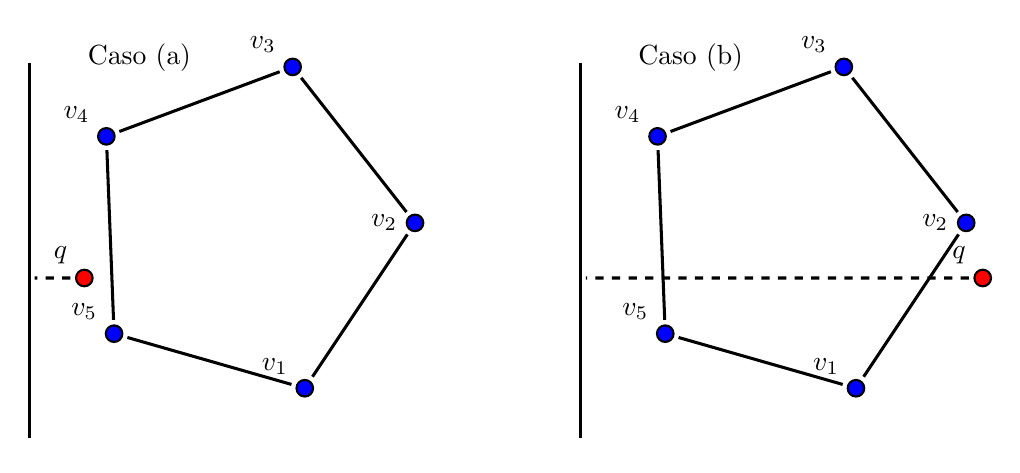
\begin{tikzpicture}[scale=0.70]
      %%%%%%%%%%%% Caso (a)
      \node(0) [blueV, label=150:$v_{1}$] at (0, 0){};
      \node(1) [blueV, label=180:$v_{2}$] at (2, 3){};
      \node(2) [blueV, label=150:$v_{3}$] at (-0.22, 5.83){};
      \node(3) [blueV, label=150:$v_{4}$] at (-3.6, 4.57){};
      \node(4) [blueV, label=150:$v_{5}$] at (-3.46, 0.99){};
      \node(5) [redV, label=150:$q$] at (-4, 2){};
      \draw[edge] (0) to (1);
      \draw[edge] (1) to (2);
      \draw[edge] (2) to (3);
      \draw[edge] (3) to (4); 
      \draw[edge] (4) to (0);
      \draw[edgeDotted] (5) to (-5,2);
      \draw[edge] (-5, -1) to (-5, 6);
      \node (L) at (-3,6){Caso (a)};
      %%%%%%%%%%%% Caso (b)      
      \begin{scope}[xshift=10cm]
        \node(0) [blueV, label=150:$v_{1}$] at (0, 0){};
        \node(1) [blueV, label=180:$v_{2}$] at (2, 3){};
        \node(2) [blueV, label=150:$v_{3}$] at (-0.22, 5.83){};
        \node(3) [blueV, label=150:$v_{4}$] at (-3.6, 4.57){};
        \node(4) [blueV, label=150:$v_{5}$] at (-3.46, 0.99){};
        \node(5) [redV, label=150:$q$] at (2.3, 2){};
        \draw[edge] (0) to (1);
        \draw[edge] (1) to (2);
        \draw[edge] (2) to (3);
        \draw[edge] (3) to (4); 
        \draw[edge] (4) to (0);
        \draw[edgeDotted] (5) to (-5,2);
        \draw[edge] (-5, -1) to (-5, 6);
        \node (L) at (-3,6){Caso (b)};
      \end{scope}
    \end{tikzpicture}
    %%%%%%%%%%%% Caso (c)
    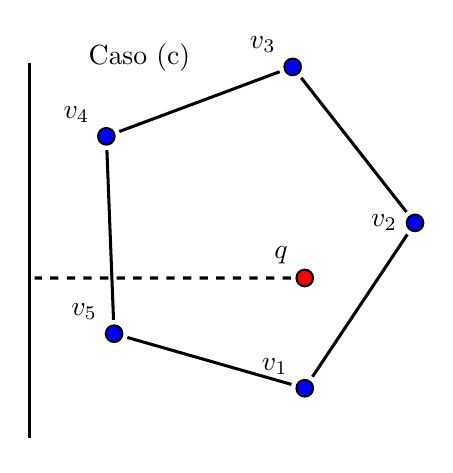
\begin{tikzpicture}[scale=0.70]
      \node(0) [blueV, label=150:$v_{1}$] at (0, 0){};
      \node(1) [blueV, label=180:$v_{2}$] at (2, 3){};
      \node(2) [blueV, label=150:$v_{3}$] at (-0.22, 5.83){};
      \node(3) [blueV, label=150:$v_{4}$] at (-3.6, 4.57){};
      \node(4) [blueV, label=150:$v_{5}$] at (-3.46, 0.99){};
      \node(5) [redV, label=150:$q$] at (0, 2){};
      \draw[edge] (0) to (1);
      \draw[edge] (1) to (2);
      \draw[edge] (2) to (3);
      \draw[edge] (3) to (4); 
      \draw[edge] (4) to (0);
      \draw[edgeDotted] (5) to (-5,2);
      \draw[edge] (-5, -1) to (-5, 6);
      \node (L) at (-3,6){Caso (c)};
    \end{tikzpicture}
  \end{figure}
  %%%%%%%%%%%%%%%%%%%%%%%%%%%%%%%%%%%%%%%%%%%%%%%%%%%%%%%%%%%%%%%%%%%%%%%%%%
  \textbf{Obs.} Encontrar $q$ respecto a los puntos de $P$ se realiza en $\mathcal{O}(\log n)$.
  Producir las recta y encontrar las intersecciones lo realizamos en $\mathcal{O}(1)$. \newline
  
  ¿Por qué será cierto que lo anterior es suficiente? R./ Sabemos que $P$ es convexo,
  entonces toda línea trazada puede cortar a $P$ en a lo más $2$ puntos. Además, como
  la proyección siempre es a la izquierda podemos tomar como referencia los puntos de
  corte respecto al polígono\footnote{Es simple plantear un pequeño sistemas de ecuación que
  me indique en cuántos puntos se corta respecto a $\ell$, todo esto en $\mathcal{O}(1)$.}.
  En otro caso, podemos considerar una orientación distinta para la línea en la que proyectaremos
  $\ell$.\newline
  
  \textit{Análisis de Complejidad.} La complejidad del algoritmo esta contenida en
  \[\mathcal{O}(1) + \mathcal{O}(\log n) \in \mathcal{O}(\log n)\]
\end{proof}

\textbf{2.} Se define el diámetro de un conjunto de puntos $S$ como la distancia más grande
entre cualesquiera dos puntos de $S$, denotado por $d$. Demuestra que d está formado por dos
vértices del cierre convexo de $S$. \newline

\textbf{\textit{Dem.}} Procedamos por reducción al absurdo. \newline

Supongamos que el diámetro $C(S)$ no contiene dos puntos del diámetro, entonces, para $d = xy$;
\begin{itemize}
        \item Los dos puntos de $d$ están dentro de $C(S)$.
              
              Esto implica que $d$ no es la distancia más grande entre cualesquiera dos puntos
              de $S$, pues tomando $xv$ donde $v$ es parte de la frontera de $C(S)$ tenemos que
              $||xv|| > ||xy||$. He aquí una contradicción de suponer que $x, y$ están dentro de
              $C(S)$.
        \item Los dos puntos de $d$ están fuera de $C(S)$.
              
              Esto implicaría que $C(S)$ no es el cierre convexo\footnote{Pues $y$ o $x$ queda fuere de $C(S)$ y
              contradice la definición de $C$.} de $S$ y por tanto llegamos a una contradicción.
        \item O hay un punto de $d$ dentro ($x$) y otro fuera ($y$) de $C(S)$.
              
              Esto implicaría que $C(S)$ no es el cierre convexo de $S$ y por tanto hemos llegado a una contradicción.
\end{itemize}
Los casos anterior muestran que $d$ esta formado por dos vértices del cierre convexo. \hfill $\square$

\newpage

%%%%%%%%%%%%%%%%%%%% Problema02:
\textbf{3.} Demuestra que cualquier polígono admite una triangulación,
incluso si el polígono tiene hoyos.\newline

\begin{proof}
  Para este ejercicio basta exhibir un algoritmo que genere la triangulación
  del polígno con hoyos. La idea será separar nuestro polígono en polígonos
  sin hoyos y triangularlos por separado. A continuación se exhibe el algoritmo
  deseado:
  \begin{enumerate}
  \item Ordenemos nuestros puntos. Esto lo realizamos en $\mathcal{O}(n \log n)$.
  \item Realizamos un barrido de línea para encontrar los hoyos. Este barrido
    nos tomará $\mathcal{O}(n)$, y detectaremos hoyos cuando el estado de la
    línea nos indique que hay al menos $4$ aristas en su posición y conforme
    el barrido avance esto se sigue cumpliendo hasta que eventualmente llegamos
    a que $2$ de los (al menos) $4$ segmentos que siempre estuvieron en el estado
    de la línea (no necesariamente los mismos segementos), siempre fueron ``internos''
    de los otros segmentos (siempre estuvieron ``entre ellos'').

    Una manera de hacer esto sería coloreando las aristas, si en un punto el estado
    de la línea me indica que las trayectorias formadas hasta el momento (con el
    avance de la línea) y coloreadas de distinto color se unen, entonces cambio el
    color a la trayectoria más pequeña. Si una trayectoria núnca se unió y además
    forma un ciclo interno al polígono, entonces este es un hoyo. \textbf{Obs.} Tomar
    esta idea sin mayor cuidado nos puede llevar a una complejidad cuadrada (aquí
    podemos hacer uso de la estrategia usada en el agoritmo de  Borůvka-Kruskal
    para encontrar ciclos y agrupar).
  \item Ahora que hemos encontrado los ciclos, podemos con gran facilidad segmentar
    nuestro polígono en nuevos polígonos sin hoyos. Para esto;
    \begin{enumerate}
    \item tomamos una arista del hoyo $O_i$, digamos $e$, entonces unimos los extremos
      de $e$ con los vértices más cercanos en el polígono y verificamos si estas nuevas
      aristas son ``estrictamente internas al polígono'' o no. En caso de que sí, entonces
      serán parte de nuestra subdivisión, en otro caso la descartamos. Esto lo podemos
      hacer con ayuda de un nuevo barrido y nos toma $\mathcal{O}(n)$ barrer nuestros puntos
      y $\mathcal{O}(n)$ realizar las comparaciones para encontrar las nuevas aristas para
      nuestra subdivisión. Si el número de aristas de $O_i$ es lineal respecto al número de vértices
      en el polígono, entonces tendremos que hacer $\mathcal{O}(n^2)$ comparaciones. De lo
      anterior tenemos una subdivisión.
    \end{enumerate}
  \item Ahora aplicamos el algoritmo de triangulación visto en clase a cada parte de la subdivisón
    encontrada.
  \end{enumerate}
  \textit{Análisis de complejidad.} La complejidad de este algoritmo esta contenida en
  \[\mathcal{O}(n + k\cdot \log n) + \mathcal{O}(n) + \mathcal{O}(n \log n) + \mathcal{O}(n^2) = \mathcal{O}(n^2).\]
  
  Como el algoritmo anterior nos regresa una triangulación de nuestro polígno con hoyos, entonces
  hemos mostrado lo requerido.
\end{proof}

\newpage

%%%%%%%%%%%%%%%%%%%% Problema02:
\textbf{4.} Un árbol de rango en un conjunto de $n$ puntos en el plano requiere
$\mathcal{O}(n log n)$ de almacenamiento. Uno podría reducir los requisitos de
almacenamiento almacenando estructuras asociadas solo con un subconjunto de los
nodos en el árbol principal.

\begin{itemize}
\item Supongamos que sólo los nodos con profundidad $0, 2, 4, 6, \dotsm$ tienen
  una estructura asociada. Muestre cómo se puede adaptar el algoritmo de consulta
  para responder consultas correctamente.
\item Analice los requisitos de almacenamiento y el tiempo de consulta de dicha
  estructura de datos.
\end{itemize}

$\rhd$ \textbf{Solución:} Para este problema dividamos la solución en dos posibles
opciones:
\begin{enumerate}
\item ¿Cómo adaptamos nuestro árbol de rangos para que cumpla lo requerido en el primer
  punto? Como sabemos que un árbol, al menos, tendrá una raíz y las estructuras estarán
  ``colgadas'' de niveles pares. Entonces, la información respecto de $Y$ de los niveles
  impares estarán contenidas en el árbol colgado en su nivel par, inmediato, anterior.
  \newline
  
  Así, las consultas para los niveles pares se quedan exactamente iguales. Para los niveles
  impares consultamos respecto de $X$ y hacemos ``bracktraking'' al nivel par, inmediato,
  anterior para terminar la consulta en la estructura colgada en el nodo de ese nivel.
\item \textit{Análisis de almacenamiento.} El almacenamiento, aunque a primera vista se reduce
  en la cantidad de niveles pares, realmente las estructuras que estaban colgadas en estos niveles
  ahora formarán parte de las estructuras en niveles pares. El ahorro de almacenamiento es $\mathcal{O}(1)$,
  pues solo nos ahorramos las raíces de los niveles impares (que son, normalmente, hojas de los niveles
  pares).\newline
  
  \textit{Análisis de tiempo de consulta.} El tiempo de consulta para un elemento en un nivel par es el mismo,
  para un elemento en un nivel impar es el mismo en términos globales, pues el ``backtraking'' lo realizamos
  en tiempo $\mathcal{O}(1)$ y la consulta en la estructura ``colgada'' sigue siendo $\mathcal{O}(\log n) + k$.
  Como la consulta en árbol respecto a $X$ (árbol grande) es $\mathcal{O}(\log n)$, concluimos una
  complejidad de consulta en $\mathcal{O}(\log^2 n)$
\end{enumerate}

\hfill $\lhd$

\newpage

%%%%%%%%%%%%%%%%%%%% Problema05:
\textbf{5.} Se pueden utilizar las estructuras de búsqueda de rangos ortogonales para determinar
si un punto particular $(a, b)$ está en un conjunto dado, haciendo una consulta al rango
$[a : a] \times [b : b]$.
\begin{enumerate}
\item[$a$)] Prueba qué hacer una consulta así en un árbol $Kd$ toma tiempo $\mathcal{O}(\log n)$.
\item[$b$)] ¿Cuál es la complejidad para una consulta así en un árbol de rangos?
\end{enumerate}

$\rhd$ \textbf{Solución:} Para este problema dividamos la solución en dos posibles casos:
\begin{enumerate}
\item[$a$)] Sabemos que hacer una consulta, en un árbol $Kd$, para un rango en
general nos toma $\mathcal{O}(\sqrt{n} + k)$. Sin embargo, consultar un punto
en un árbol $Kd$ sería equivalente a particionar la nuve de puntos por la mitad
y preguntarnos en qué parte queda nuestro punto distinguido, llamemosle $q$. Así,
descartamos aproximadamente la mitad de puntos en dónde no se encuentra $q$. Luego,
subdividimos nuevamente el conjunto de puntos restantes en $2$ y nos preguntamos
en qué parte se encuentra $q$ y podemos descartar la parte en la que no se encuentre.
De esta manera y recursivamente nuestro espacio de búsqueda se reduce a la mitad cada
vez, esto equivale hacer un recorrido de la raíz de nuestro árbol $kd$ hacia las hojas
en búsca del punto $q$. Como cada vez descontamos la mitad del conjunto de puntos
de búsqueda, tenemos la recurrencia $T(n) = 2T(n - 1)$ que sabemos que nos genera
un orden logarítmico en base 2. Cómo el número de consultas es igual a $1$, entonces
$k = 1 \in \mathcal{O}(1)$. Por tanto, la complejidad de esta consulta es
$\mathcal{O}(\log n)$.
\item[$b$)] En este caso, tenemos una complejidad general de $\mathcal{O}(\log^2 n + k)$,
cómo solo estamos consultando un punto y no un rango, entonces $k = 1 \in \mathcal{O}(1)$.
En la consulta debemos bajar por el árbol hasta encontrar $q.X$ y bajar su árbol ``colgado''
o su árbol asociado en $y$, hacer esto es igual a $\log m$ dónde $m$ es la altura del árbol
asociado con $m \not= n$, pues cada nivel y nodo tiene un árbol compacto de tamaño constante.
Por tanto, la complejidad esta contenida en $\mathcal{O}(\log m \cdot \log n) = \mathcal{O}(\log n)$
con $m$ constante respecto de $n$.

\end{enumerate}
\hfill $\lhd$

\newpage

%%%%%%%%%%%%%%%%%%%% Problema06:
\textbf{6.} En algunas aplicaciones solo nos interesa el número de puntos que caen dentro de
un rango y no reportar cada uno de ellos. En este caso nos gustaría evitar el término
$\mathcal{O}(k)$ en el tiempo de consulta.
\begin{enumerate}
\item[$a$)] Describe cómo un árbol de rangos de una dimensión puede adaptarse para que
una consulta así se pueda realizar en tiempo $\mathcal{O}(\log n)$.
\item[$b$)] Usando la solución al problema para una dimensión, describe cómo se pueden
responder consultas de conteo en rangos de $d$ dimensiones en tiempo $\mathcal{O}(\log^d n)$.
\item[$c$)] Describe cómo se puede usar la técnica de cascada para mejorar el tiempo de
consulta en un factor $\mathcal{O}(\log n)$ para dos y más dimensiones.
\end{enumerate}

$\rhd$ \textbf{Solución:} A continuación se da solución a cada uno de los incisos:
\begin{enumerate}
\item[$a$)] La versión para una dimensión sería bastante simple, y de hecho sería
  como un árbol binario de búsqueda balanceado, pues basta con preservar el árbol
  general sin los árboles ``colgados'' que tiene el árbol de búsuqeda ortogonal.
  \newline
  
  La manera de ahorrar $\mathcal{O}(k)$ durante la búsqueda de rango, sería no recorrer las
  hojas del rango encontrado. Pues, basta con realizar dos recorridos hacia abajo desde la
  raíz, uno para encontrar la cota inferior del rango y otro para encontrar la cota superior.
  Así, y por la propiedad de tener mayores a la derecha y menores a la izquierda concluimos
  que las hojas entre las seleccionadas forman parte del rango.
\item[$b$)] De la misma manera, que en el caso de una dimensión, nos ahorramos $\mathcal{O}(k)$
  al no recorrer las hojas que quedan dentro del rango. Para generalizar a $d$ dimensiones basta
  reproducir la idea de los árboles ``colgados'', pues cada nodo que no sea hoja tendrá, inicialmente
  una referencia al árbol con coordenadas en $Y$. Luego los árboles con coordenadas en $Y$ tendrán
  colgados árboles con coordenadas en $Z$, y así de manera recursiva. Cuándo se requiera obtener
  el rango bastará con bajar por el árbol principal y recorrer cada árbol asociado de manera
  recursiva para inspeccionar que efectivamente el punto quede dentro del rango requerido.
  Cómo recorremos $\log n$ el árbol principal y por cada nodo distinto a una hoja recorremos
  su árbol asociado y a su vez los asociados recursivamente, entonces tenemos una complejidad
  de $k \cdot \log n$ dónde $k = \log m \cdot \log m' \dotsm \log m^{\dotsm} \approx \log^{d - 1} n$
  y concluimos que la complejidad en general por recorrido para encontrar un punto en el rango
  es de $\mathcal{O}(\log^d n)$.\newline
  
  Como esto se tiene que hacer para el punto ``menor'' en el rango y para el punto ``mayor''
  en el rango,  entonces tenemos una complejidad contenida en
  \[2 \cdot \mathcal{O}(\log^d n) \in \mathcal{O}(\log^d n).\]
\item[$c$)] 
\end{enumerate}
\hfill $\lhd$


\newpage
%%%%%%%%%%%%%%%%%%%% Problema07:
\textbf{7.} Da un algoritmo que calcule en tiempo $O(n \log n)$ una diagonal que divida un
polígono simple con $n$ vértices en dos polígonos simples cada uno con a lo más
$\lfloor \frac{2n}{3} \rfloor + 2$ vártices. \textbf{Hint}: Usa la gráfica dual de la triangulación.
\newline

$\rhd$ \textbf{Solución:} A continuación se exhibe un algoritmos que resuelve este problema
\begin{enumerate}
\item Obntener la triangulación de nuestro polígono. Esto lo realizamos en $\mathcal{O}(n \log n)$
  con el algoritmo visto en clase.
\item Sabemos que toda triangulación tiene $n - 3$ aristas y por tanto nuestra gráfica dual que
  se formará a partir de cada arista interna será de un orden $\mathcal{O}(n)$. Entonces, la
  construcción de la gráfica dual nos toma $\mathcal{O}(n)$. Además, la gráfica dual es un árbol.
\item Encontramos los puntos más lejanos en una gráfica. Esto, por algoritmos $I$ sabemos que
  lo podemos hacer en $\mathcal{O}(n)$ para un árbol. La técnica se basa en ``colgar'' el árbol
  por medio de un recorrido a profundidad desde la raíz hasta la hoja de mayor profundidad y
  tomar esa hoja como la nueva raíz y volver a recorrer hasta la hoja más profunda.
\item  Recorrer la gráfica dual iniciando desde cada uno de los puntos más lejanos. Eligimos una
  orientación y siempre seguimos esta orientación (La orientación, la podemos tener con DCEL) para
  el reccorido. Así evitaremos dividir el polígono en más de $2$ polígonos nuevos. Esto lo hacemos
  en $\mathcal{O}(n)$, pues el orden de las aristas de nuestra gráfica dual es lineal.
\item Durante cada recorrido colorearemos los vértices del triángulo en el que estemos, todos
  del mismo color. En el momento que hayamos coloreado, exactamente $\lfloor \frac{2n}{3} \rfloor + 2$
  vértices. Entonces regresamos la arista $e_T$ de la triangulación por la que fue creada la arista
  siguiente a la última hasta haber coloreado los  $\lfloor \frac{2n}{3} \rfloor + 2$ vértices.
  Esto lo hacemos en $3 \cdot \left( \lfloor \frac{2n}{3} \rfloor + 2\right)$ pasos que obedece
  a un orden líneal.\newline
  
  ¿Con cuál recorrido nos quedamos? Con el que llegue primero a colorear los $\lfloor \frac{2n}{3} \rfloor + 2$
  vértices y cumpla que la arista divide al polígono en las características deseadas.\newline

  \textbf{Obs.} Podríamos hacer una versión con $\lfloor \frac{n}{3} \rfloor - 2$ tomandolo por cota.
\end{enumerate}
Al final, $e_T$ es la diagonal búscada.\newline

\textit{Análisis de la complejidad.} La complejidad del algoritmo esta contenida en
\[\mathcal{O}(n \log n) + \mathcal{O}(n) = \mathcal{O}(n \log n).\]
\hfill $\lhd$

\newpage

%%%%%%%%%%%%%%%%%%%% Problema07:
\textbf{8.} Sea S un conjunto de $n$ puntos en el plano y $A$ una subdivisión plana con $\mathcal{O}(n)$
regiones:
\begin{itemize}
\item Muestra que toma $\mathcal{O}(n \log n)$ localizar los puntos de $S$ en $A$.
\item Sea $T$ una triangulación de $S$, ¿cómo podría ayudar esta información para
localizar los puntos de $S$ en $A$? Muestra que a pesar de tener la triangulación
de $S$, la cota sigue siendo logarítmica.
\end{itemize}

\begin{proof}
  Para probar los incisos anteriores basta exhibir un algoritmo que encuentre los puntos
  requeridos en $\mathcal{O}(n \log n)$. A continuación se solucionan los incisos anteriores,
  esto es
  \begin{itemize}
  \item Usando el algoritmo de David Kirkpatrik visto en clase, podemos calcular la localización
    de cada uno de los puntos. Localizar un punto por medio de este algoritmo nos toma $\mathcal{O}(\log n)$,
    cómo buscamos localizar $n$ puntos, entonces tenemos que aplicar este algoritmo $n$ veces. Así,
    localizar la región de $A$ en la que esta contenido cada punto nos cuesta $\mathcal{O}(n \log n)$.
  \item Tener una triangulación en los puntos nos ayudaría a ahorrar algunas subdivisiones, sin embargo,
    habría que verificar que nuestra subdivisión $A$ más $T$ siga siendo plana, por lo que no necesariamente
    ahorramos complejidad. Incluso, si ahorraramos complejidad esta sería pequeña, de hecho sería de tamaño
    constante y nuestro algoritmo seguiría necesitando de $\mathcal{O}(n \log n)$ para localizar todos
    los puntos, pues los demás pasos se siguen teniendo (ir quitando los de vértices de menor grado $< 8$
    e ir retriangulando, luego regresarnos por medio de nuestro árbol).
  \end{itemize}
\end{proof}

\end{document}
